\documentclass[xcolor=pdftex,romanian,colorlinks]{beamer}
%\documentclass[xcolor=pdftex,handout,romanian,colorlinks]{beamer}

\usepackage[export]{adjustbox}
\usepackage{../sty/tslides}
\usepackage[all]{xy}
\usepackage{pgfplots}
\usepackage{flowchart}
\usepackage{todonotes}
\usepackage{multicol}  
\usetikzlibrary{arrows,positioning,calc}
\lstset{language=Haskell}
\lstset{escapeinside={(*@}{@*)}}
\PrerenderUnicode{ăĂîÎȘșȚțâÂ}
\usepackage{amsmath}


%\usepackage{xcolor}
%\definecolor{IntensColor}{HTML}{2E86C1}
%\definecolor{StateTransition}{HTML}{D6EAF8}
%\definecolor{MedianLightOrange}{RGB}{216,178,92}
%\definecolor{Orchid}{HTML}{8E44AD}
%\definecolor{True}{HTML}{229954}
%\definecolor{False}{HTML}{CB4335}


\usepackage{proof}
\usepackage{multirow}
\usepackage{alltt}
\usepackage{mathpartir}
\usepackage{ulem}

\newcommand{\structured}[1]{#1}

\definecolor{IntensColor}{HTML}{2E86C1}
\definecolor{StateTransition}{HTML}{D6EAF8}
\definecolor{MedianLightOrange}{RGB}{216,178,92}
\definecolor{Orchid}{HTML}{8E44AD}
\definecolor{True}{HTML}{229954}
\definecolor{False}{HTML}{CB4335}

\newcommand{\cin}[1]{{\color{cobalt} #1}}
\newcommand{\sel}[1]{{\color{Orchid} #1}}

\newcommand{\intens}[1] {{\color{IntensColor} #1}}
\newcommand{\exe}[1] {{\color{True} #1}}

\newcommand{\la}{\lambda}

\setlength{\leftmargini}{0pt}

\newcommand{\app}[2]{#1\, #2}
\newcommand{\abs}[2]{\lambda #1.\,#2}

\newcommand{\type}[2]{{\color{True}#1\hspace{-.05cm}:}\,{\color{Orchid}#2}}

\newcommand{\sub}[3]{#1\langle#2/#3\rangle}
\newcommand{\subt}[3]{#1[#2/#3]}
\newcommand{\equiva}{=_\alpha}

\newcommand{\trueL}{\mathbf{T}}
\newcommand{\falseL}{\mathbf{F}}
\newcommand{\notL}{\mathbf{not}}
\newcommand{\andL}{\mathbf{and}}
\newcommand{\orL}{\mathbf{or}}
\newcommand{\ifL}{\mathbf{if}}
\newcommand{\boolL}{\mathbf{bool}}

\newcommand{\maybeL}{\mathbf{maybe}}
\newcommand{\nothingL}{\mathbf{Nothing}}
\newcommand{\justL}{\mathbf{Just}}
\newcommand{\Maybe}[1]{\mathop{\mathbf{Maybe}}{#1}}

\newcommand{\foldrL}{\mathbf{foldr}}
\newcommand{\nilL}{\mathbf{Nil}}
\newcommand{\consL}{\mathbf{Cons}}
\newcommand{\ListL}[1]{\mathop{\mathbf{List}}{#1}}

\newcommand{\unpairL}{\mathbf{uncons}}
\newcommand{\pairL}{\mathbf{Pair}}
\newcommand{\firstL}{\mathbf{first}}
\newcommand{\secondL}{\mathbf{second}}
\newcommand{\Pair}[2]{\mathop{\mathop{\mathbf{Pair}}{#1}}{#2}}

\newcommand{\succL}{\mathbf{Succ}}
\newcommand{\zeroL}{\mathbf{Zero}}
\newcommand{\iterateL}{\mathbf{iterate}}
\newcommand{\addL}{\mathbf{add}}
\newcommand{\mulL}{\mathbf{mul}}
\newcommand{\expL}{\mathbf{exp}}
\newcommand{\isZero}{\mathbf{isZero}}
\newcommand{\pred}{\mathbf{pred}}
\newcommand{\factL}{\mathbf{fact}}

\newcommand{\BoolT}{\ensuremath{\texttt{Bool}}}
%\newcommand{\BoolT}{\ensuremath{\texttt{Bool}}}
\newcommand{\ifT}[3]{\mathrm{if}\ #1\ \mathrm{then}\ #2\ \mathrm{else}\ #3}

\newcommand{\UnitT}{\ensuremath{\texttt{Unit}}}
\newcommand{\unit}{\mathrm{unit}}

\newcommand{\VoidT}{\ensuremath{\texttt{Void}}}
\newcommand{\void}{\mathrm{void}}


\newcommand{\ProductT}[2]{#1 \times #2}
\newcommand{\PairL}[2]{\langle #1,#2\rangle}
\newcommand{\ProjOne}[1]{fst\ #1}
\newcommand{\ProjTwo}[1]{snd\ #1}

\newcommand{\SumT}[2]{#1 + #2}
\newcommand{\Left}[1]{\mathrm{Left}\ #1}
\newcommand{\Right}[1]{\mathrm{Right}\ #1}
\newcommand{\Case}[3]{\mathrm{case}\ #1\ \mathrm{of}\ #2\ ;\ #3}

%----------------------------------------------

\newcommand{\SSnot}{\terminal{not}}

\newcommand{\Sand}{\terminal{and}}
\newcommand{\Sor}{\terminal{or}}
\newcommand{\Splus}{\terminal{+}}
\newcommand{\Smul}{\terminal{*}}
\newcommand{\Ssucc}{\terminal{S}}
\newcommand{\Spow}{\terminal{pow}}
\newcommand{\Spred}{\terminal{pred}}
\newcommand{\Seq}{\terminal{eq}}
\newcommand{\Sneq}{\terminal{neq}}

\newcommand{\SisZero}{\terminal{isZero}}
\newcommand{\Slte}{\terminal{<=}}
\newcommand{\Sgte}{\terminal{>=}}
\newcommand{\Slt}{\terminal{<}}
\newcommand{\Sgt}{\terminal{>}}
\newcommand{\Spair}{\terminal{pair}}
\newcommand{\Sfst}{\terminal{fst}}
\newcommand{\Ssnd}{\terminal{snd}}
\newcommand{\Sminus}{\terminal{-}}

\newcommand{\Snull}{\terminal{null}}
\newcommand{\Scons}{\terminal{cons}}
%\newcommand{\c sead}{\terminal{head}}
\newcommand{\SisNull}{\terminal{?null}}
\newcommand{\Stail}{\terminal{tail}}
\newcommand{\Ssum}{\terminal{sum}}
\newcommand{\Sfoldr}{\terminal{foldr}}
\newcommand{\Smap}{\terminal{map}}
\newcommand{\Sfilter}{\terminal{filter}}

\newcommand{\const}[1]{\triangleright {\color{False} #1}}

\newcommand{\egf}[1]{\stackrel{\cdot}{=}_{#1}}

\newcommand{\Conf}[2]{\ensuremath{\langle #1\ ,\ #2\rangle}}
\newcommand{\plus}[1] {{\color{True} #1}}
\newcommand{\te}[1]{\mbox{\texttt{#1}}}

\newcommand{\vexp}{\ensuremath{\mathbb{E}}}
\newcommand{\bexp}{\ensuremath{\mathbb{B}}}
\newcommand{\cmd}{\ensuremath{\mathbb{C}}}

\definecolor{section-color}{HTML}{23373b} %mDarkTeal
%\AtBeginSection[]{
%  \begin{frame}
%  \vfill
%  \centering
%  \begin{beamercolorbox}[sep=8pt,center,shadow=true,rounded=true]{title}
%    \usebeamerfont{title}\insertsectionhead\par%
%  \end{beamercolorbox}
%  \vfill
%  \end{frame}
%}



\title[FLP]{Fundamentele limbajelor de programare}
\subtitle{C09}
\date{}


\begin{document}
\begin{frame}
  \titlepage
\end{frame}

\setlength{\leftmargini}{12pt}


%================================================
\section{\color{section-color}Programare logică \& Prolog}
%================================================

%-------------------------------------------------------------
\begin{frame}{Programare logică}


\intens{Programarea logică} este o paradigmă de programare 
	bazată pe logică.
	
	\vspace{.2cm} 
Unul din sloganurile programării logice:
	\vspace{-.2cm}
	\begin{center}
	\href{https://www.doc.ic.ac.uk/~rak/papers/History.pdf}{\intens{\textbf{Program = Logică + Control}}}  \quad {\em (R. Kowalski)}	
	\end{center} 
	
	\vspace{.2cm}
Programarea logică poate fi privită ca o deducție controlată.	
	
	\vspace{.2cm} 
Un \intens{program} scris într-un limbaj de programare logică este
	\vspace{-.2cm}
	\begin{center}
	\intens{o listă de formule într-o logică}
	\end{center}
		\vspace{-.2cm}
	ce exprimă fapte și reguli despre o problemă.
\end{frame}

%-------------------------------------------------------------
\begin{frame}{Programare logică}

	\vspace{.2cm} 
 Exemple de limbaje de programare logică: 
		\begin{itemize}
			\item \intens{Prolog}
			\item \intens{Answer set programming (ASP)}
			\item \intens{Datalog}
		\end{itemize}

\end{frame}



%---------------------------------------------------------------------
\begin{frame}{Programare logică - în mod idealist}
\begin{itemize}
	\item Un \intens{"program logic"} este o colecție de proprietăți presupuse (sub formă de formule logice) despre lumea programului.
	\medskip
	\item Programatorul furnizează și o proprietate (o formula logică) care poate să fie sau nu adevărată în lumea respectivă (\intens{întrebare, \intens{query}}).
	\medskip
	\item Sistemul determină dacă proprietatea aflată sub semnul întrebării este o consecință a proprietăților presupuse în program.
	\medskip
		\item Programatorul nu specifică metoda prin care sistemul verifică dacă întrebarea este sau nu consecință a programului.
\end{itemize}
\end{frame}
%---------------------------------------------------------------------

%---------------------------------------------------------------------
\begin{frame}{Exemplu de program logic}
\begin{center}
\begin{tabular}{rcl}
\texttt{oslo} & $\to$ & \texttt{windy} \\[.5em]
\texttt{oslo} & $\to$ & \texttt{norway} \\[.5em]
\texttt{norway} & $\to$ & \texttt{cold} \\[.5em]
\texttt{cold $\wedge$ windy} & $\to$ & \texttt{winterIsComing} \\[.5em]
& & \texttt{oslo}\\
\end{tabular}
\end{center}
\bigskip 

\textbf{\color{True} Exemplu de întrebare.}
Este adevărat \intens{\texttt{winterIsComing}}?
\end{frame}
%---------------------------------------------------------------------

%---------------------------------------------------------------------

\begin{frame}{Prolog}

\vfill\begin{itemize}
	\item bazat pe logica clauzelor Horn
	\item semantica operațională este bazată pe rezoluție
	\item este Turing complet
\end{itemize}

\intens{Program:}
\vspace{-.4cm}
\begin{alltt}
windy :- oslo. \\
norway :- oslo. \\
cold :- norway. \\
winterIsComing :- windy, cold. \\
oslo. \\
\end{alltt}


\intens{Intrebare:}
\vspace{-.4cm}
\begin{alltt}
?- winterIsComing.\\
true
\end{alltt}

\underline{\url{http://swish.swi-prolog.org/}}
\end{frame}
%---------------------------------------------------------------------

%%------------------------------------------------
%\begin{frame}
%  \vfill
%  \centering
%
%TODO
%
%\textbf{\large \alert{Quiz time!}}
%
%
\includegraphics[scale=.35]{../Quiz/C06-Q1.png}
%
% \url{https://www.questionpro.com/t/AT4NiZrHFn}
%  \vfill
%\end{frame}



%---------------------------------------------------------------------
\begin{frame}{Sintaxă: constante, variabile, termeni compuși}

\bigskip

\begin{itemize}
	
		
		  \item \intens{Atomi}: \texttt{brian, 'Brian Griffin', 
		  brian\_griffin}
		  \bigskip
		  \item \intens{Numere}: \texttt{23, 23.03,-1}
		
		\medskip
		
		\intens{Atomii} și \intens{numerele} sunt \intens{constante}.
		\medskip
		\item \intens{Variabile}: \texttt{X, Griffin, \_family}

		\bigskip
			\item Termeni \intens{compuși}: \texttt{father(peter, stewie\_griffin)},
			
\hspace*{1cm}\texttt{and(son(stewie,peter), daughter(meg,peter))}

\begin{itemize}
\item[-]   forma generală:	\intens{atom(termen,$\ldots$, termen)}
 \item[-]  atom-ul care denumește termenul se numește \intens{functor}		      	
			      	
\item[-] numărul de argumente se numește \intens{aritate}			      	\end{itemize}
\end{itemize}

\end{frame}


%---------------------------------------------------------------------
\begin{frame}{Sintaxă Prolog}

\textbf{\color{True} Exercițiu.} Care din următoarele șiruri de caractere sunt \intens{constante} și care sunt \intens{variabile} în Prolog?

\begin{itemize}
	\item vINCENT \onslide<2->{-- \intens{constantă}}
	\item Footmassage \onslide<2->{-- \alert{variabilă}} 
	\item variable23 \onslide<2->{-- \intens{constantă}}
	\item Variable2000 \onslide<2->{-- \alert{variabilă}} 
	\item big\_kahuna\_burger \onslide<2->{-- \intens{constantă}}
	\item 'big  kahuna  burger' \onslide<2->{-- \intens{constantă}}
	\item big  kahuna  burger \onslide<2->{-- {\color{False} nici una, nici alta}}
	\item 'Jules' \onslide<2->{-- \intens{constantă}}
	\item \_Jules \onslide<2->{-- \alert{variabilă}} 
	\item '\_Jules' \onslide<2->{-- \intens{constantă}}
\end{itemize}

\end{frame}

%---------------------------------------------------------------------
\begin{frame}[fragile]{Program  în Prolog = bază de cunoștințe}

\textbf{\color{True} Exemplu.} Un program în Prolog:
\begin{verbatim}
father(peter,meg). 
father(peter,stewie).

mother(lois,meg). 
mother(lois,stewie).

griffin(peter).
griffin(lois).

griffin(X) :- father(Y,X),  griffin(Y).
\end{verbatim}

Un program  în Prolog este o \intens{bază de cunoștințe} (\intens{K}nowledge \intens{B}ase).
\end{frame}

%---------------------------------------------------------------------

\begin{frame}[fragile]{Program  în Prolog = mulțime de predicate}

Practic, g\^{a}ndim un program  în Prolog ca o mulțime de \intens{predicate}  cu ajutorul cărora descriem {\it lumea} ({\it universul}) programului respectiv.
 
\textbf{\color{True} Exemplu.}
\begin{columns}
\begin{column}{.5\textwidth}
\vspace{-.2cm}
\begin{verbatim}
father(peter,meg). 
father(peter,stewie).

mother(lois,meg). 
mother(lois,stewie).

griffin(peter).
griffin(lois).

griffin(X) :- father(Y,X),  griffin(Y).
\end{verbatim}
\end{column}
\begin{column}{.3\textwidth}
\intens{\textbf{Predicate:}}\\
\intens{father/2}\\
\intens{mother/2}\\
\intens{griffin/1}
\end{column}
\end{columns}

\end{frame}
%----------------------------------------------------


\begin{frame}{Un program în Prolog}

\begin{center}
%Un program în Prolog răspunde la întrebări.

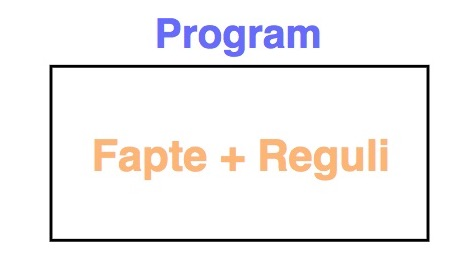
\includegraphics[scale=.3]{images/Prolog1}


\end{center}


\end{frame}
%---------------------------------------------------------------------


%---------------------------------------------------------------------
\begin{frame}{Program }

\begin{itemize}
	\item Un \intens{program} în Prolog este format din \intens{reguli} de forma
	\begin{center}
	\intens{Head :- Body.}
	\end{center} 
	\medskip
	
\item \intens{Head} este un predicat, iar \intens{Body} este o secvență de predicate separate prin virgulă.

\medskip
	
\item Regulile fără \texttt{Body} se numesc \intens{fapte}.
\end{itemize}

\medskip  
\textbf{\color{True} Exemple.}
\vspace{-.2cm}
\begin{itemize}
	\item  Exemplu de regulă: \\ \texttt{griffin(X) :- father(Y,X),  griffin(Y).}
	\item  Exemplu de fapt: \\ \texttt{father(peter,meg).}
\end{itemize}

\end{frame}
%---------------------------------------------------------------------


\begin{frame}{Interpretarea din punctul de vedere al logicii}

Operatorul \intens{\textbf{:-}} este implicația logică \intens{$\leftarrow$}.

\vspace{.2cm}
\textbf{\color{True} Exemplu.}
\texttt{comedy(X) :- griffin(X).}
\smallskip

\intens{dacă} \texttt{griffin(X)} \intens{este adevărat, atunci} 
\texttt{comedy(X)} \intens{este adevărat.}

 
\vspace{.6cm}
Virgula \intens{,} este conjuncția \intens{$\wedge$}.

\vspace{.2cm}
\textbf{\color{True} Exemplu.}
\texttt{griffin(X) :- father(Y,X),  griffin(Y).}

\smallskip

\intens{dacă} \texttt{father(Y,X)} \intens{și} \texttt{griffin(Y)}  \intens{sunt adevărate,}

\intens{atunci} \texttt{griffin(X)} \intens{este adevărat.}
\end{frame}

\begin{frame}{Interpretarea din punctul de vedere al logicii}

Mai multe reguli cu \intens{același Head} definesc același predicat, între definiții fiind un \intens{sau} logic. 


\vspace{.2cm}
\textbf{\color{True} Exemplu.}
\vspace{-.2cm}
\begin{alltt}
comedy(X) :- family\_guy(X).\\
comedy(X) :- south\_park(X).\\
comedy(X) :- disenchantment(X).\\
\end{alltt}
\smallskip

\intens{dacă} 
 \texttt{family\_guy(X)} \intens{este adevărat sau}
\texttt{south\_park(X)} \intens{este adevărat sau}
 \texttt{disenchantment(X)}  \intens{este adevărat,}
  
\intens{ atunci} 
\texttt{comedy(X)} \intens{este adevărat}.


\end{frame}

%---------------------------------------------------------------------

\begin{frame}{Un program în Prolog}

\begin{center}
%Un program în Prolog răspunde la întrebări.

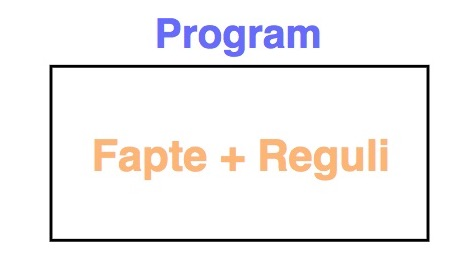
\includegraphics[scale=.3]{images/Prolog1}

\vspace*{1cm}

Cum folosim un program  în Prolog?
\end{center}


\end{frame}
%---------------------------------------------------------------------

\begin{frame}{\^Intrebări în Prolog}

\begin{center}
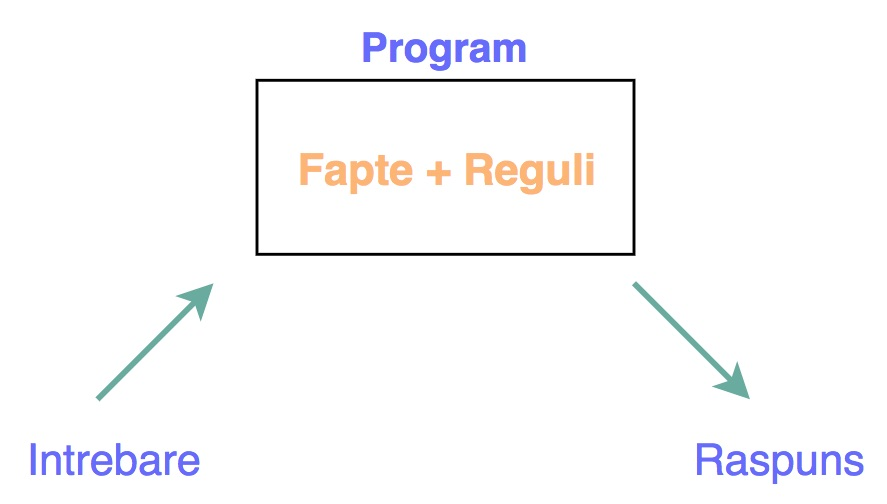
\includegraphics[scale=.3]{images/Prolog}
\end{center}

\end{frame}
%---------------------------------------------------------------------

%---------------------------------------------------------------------

\begin{frame}{\^Intrebări și ținte în Prolog}

\begin{itemize}
	\item Prolog poate răspunde la întrebări legate de consecințele relațiilor descrise într-un program în Prolog.
	\smallskip
	\item \intens{Întrebările} sunt de forma:
	\begin{center}
	\intens{\texttt{?- predicat$_1$($\ldots$),$\ldots$,predicat$_n$($\ldots$).}}
	\end{center}
	\smallskip
	\item Prolog verifică dacă întrebarea este o consecință a relațiilor definite în program.
	\smallskip
	\item Dacă este cazul, Prolog caută valori pentru variabilele care apar în întrebare astfel încât întrebarea să fie o consecință a relațiilor din program.
\smallskip	
	\item Un predicat care este analizat pentru a răspunde la o întrebare se numește \intens{țintă} (\intens{goal}).
\end{itemize}
\end{frame}
%---------------------------------------------------------------------

%---------------------------------------------------------------------

\begin{frame}{\^Intrebări în Prolog}


Prolog poate da 2 tipuri de răspunsuri:
	\begin{itemize}
		\item {\color{red} \texttt{false}} -- dacă întrebarea nu este o consecință a programului.
		\smallskip
		\item \intens{\texttt{true}} sau \intens{valori pentru variabilele din întrebare} dacă întrebarea este o consecință a programului.
	\end{itemize}

 
\begin{example}
\smallskip
\begin{columns}
\begin{column}{.4\textwidth}
 \texttt{?- griffin(meg)} \\
	  \texttt{true}
	  
\texttt{?- griffin(glenn)} \\
	  \texttt{false}
\vspace{.8cm}	
\end{column}
\begin{column}{.4\textwidth}
\texttt{?- griffin(X)} \\
	\texttt{X = petr ;} \\
	\texttt{X = lois ;} \\
	\texttt{X = meg ;} \\
	\texttt{X = stewie ;} \\
	\texttt{false} \\
\end{column}
\end{columns}
\smallskip
\end{example}
\end{frame}



%---------------------------------------------------------------------

\begin{frame}[fragile]{Cum găsește Prolog răspunsul}

Pentru a găsi un răspuns, \\ \intens{Prolog încearcă regulile în ordinea apariției lor.}

\textbf{\color{True} Exemplu.}
Să presupunem că avem programul: 
\begin{verbatim}
foo(a).  foo(b).  foo(c).
\end{verbatim}
și că punem întrebarea: \\
{\color{blue}\texttt{?- foo(X).}}\\
{\color{blue}\texttt{X = a.}}\\


Pentru a răspunde la întrebare se caută o \intens{potrivire} (\intens{unificator}) între scopul {\color{blue}\texttt{foo(X)}} și baza de cunoștințe. Răspunsul este \intens{substituția} care realizează unificarea, în cazul nostru {\color{blue}\texttt{X = a}}. 

\begin{center}
\intens{Răspunsul la întrebare este găsit prin unificare!}
\end{center}

\end{frame}


%---------------------------------------------------------------------

\begin{frame}[fragile]{Cum găsește Prolog răspunsul}

\textbf{\color{True} Exemplu.} Să presupunem că avem programul: 
\begin{verbatim}
foo(a).  foo(b).  foo(c).
\end{verbatim}
și că punem  întrebările: \\
{\color{blue}\texttt{?- foo(X).}}\\
{\color{blue}\texttt{X = a.}}\\
\medskip

{\color{blue}\texttt{?- foo(d).}}\\
{\color{red}\texttt{false}}\\
\smallskip


Dacă nu se poate face unificarea, răspunsul este 
{\color{red}{false}}.

\end{frame}
%---------------------------------------------------------------------

\begin{frame}[fragile]{Cum găsește Prolog răspunsul}


\textbf{\color{True} Exemplu.} Să presupunem că avem programul: 
\begin{verbatim}
foo(a).  foo(b).  foo(c).
\end{verbatim}
și că punem întrebarea: \\
{\color{blue}\texttt{?- foo(X).}}\\
{\color{blue}\texttt{X = a.}}\\

\smallskip 

Dacă dorim mai multe răspunsuri, tastăm \color{blue}{\texttt{;}}\\
\smallskip

{\color{blue}\texttt{?- foo(X).}}\\
{\color{blue}\texttt{X = a ;}}\\
{\color{blue}\texttt{X = b ;}}\\
{\color{blue}\texttt{X = c.}}



\end{frame}

\addtocounter{framenumber}{-1}
%------------------------------------------------------------------
\begin{frame}[fragile]{Cum găsește Prolog răspunsul}


\textbf{\color{True} Exemplu.} 
\begin{multicols}{2}
Să presupunem că avem programul: 
\begin{verbatim}
foo(a). 
foo(b). 
foo(c).
\end{verbatim}
și că punem întrebarea: \\
{\color{blue}\texttt{?- foo(X).}}
\columnbreak
\begin{figure}[h]
    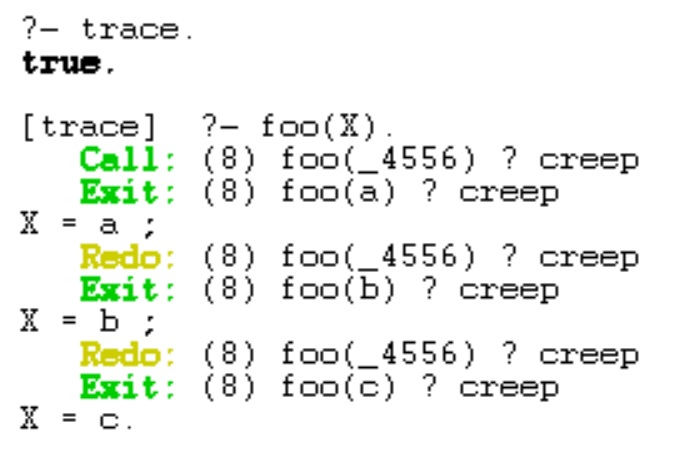
\includegraphics[width=0.4\textwidth]{images/trace1}
\end{figure}
\end{multicols}

\end{frame}

%------------------------------------------------------------------

\begin{frame}[fragile]{Cum găsește Prolog răspunsul}

Pentru a găsi un raspuns, \intens{Prolog redenumește variabilele.}

\textbf{\color{True} Exemplu.} 
\begin{multicols}{2}
Să presupunem că avem programul: 
\begin{verbatim}
foo(a). 
foo(b). 
foo(c).
\end{verbatim}
și că punem  întrebarea: \\
{\color{blue}\texttt{?- foo(X).}}
\columnbreak
\begin{figure}[h]
    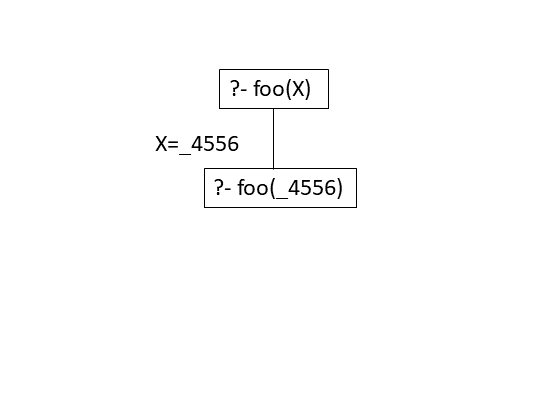
\includegraphics[width=0.4\textwidth]{images/foo1}
\end{figure}
\end{multicols}

\end{frame}

%------------------------------------------------------------------
\begin{frame}[fragile]{Cum găsește Prolog răspunsul}



\textbf{\color{True} Exemplu.} 
\begin{multicols}{2}
Să presupunem că avem programul: 
\begin{verbatim}
foo(a). 
foo(b). 
foo(c).
\end{verbatim}
și că punem întrebarea: \\
{\color{blue}\texttt{?- foo(X).}}
\columnbreak
\begin{figure}[h]
    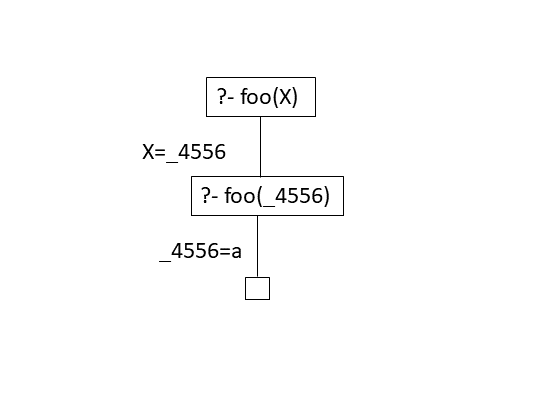
\includegraphics[width=0.4\textwidth]{images/foo2}
\end{figure}
\end{multicols}

În acest moment, a fost găsită  prima soluție: \texttt{X=\_4556=a}.
\end{frame}

%------------------------------------------------------------------
\begin{frame}[fragile]{Cum găsește Prolog răspunsul}


\textbf{\color{True} Exemplu.} 
\begin{multicols}{2}
Să presupunem că avem programul: 
\begin{verbatim}
foo(a). 
foo(b). 
foo(c).
\end{verbatim}
și că punem următoarea întrebare: \\
{\color{blue}\texttt{?- foo(X).}}
\columnbreak
\begin{figure}[h]
    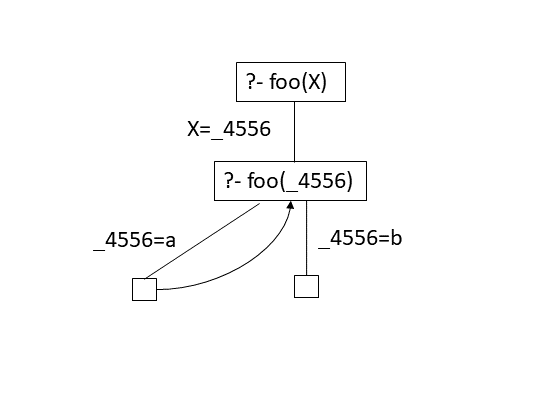
\includegraphics[width=0.4\textwidth]{images/foo3}
\end{figure}
\end{multicols}

\vspace{-.2cm}
Dacă se dorește încă un răspuns, atunci se face un pas înapoi în \intens{arborele de căutare} și se încearcă satisfacerea țintei cu o nouă valoare.
\end{frame}

%------------------------------------------------------------------
\begin{frame}[fragile]{Cum găsește Prolog răspunsul}



\textbf{\color{True} Exemplu.} 
\begin{multicols}{2}
Să presupunem că avem programul: 
\begin{verbatim}
foo(a). 
foo(b). 
foo(c).
\end{verbatim}
și că punem întrebarea: \\
{\color{blue}\texttt{?- foo(X).}}
\columnbreak

\begin{figure}[h]
    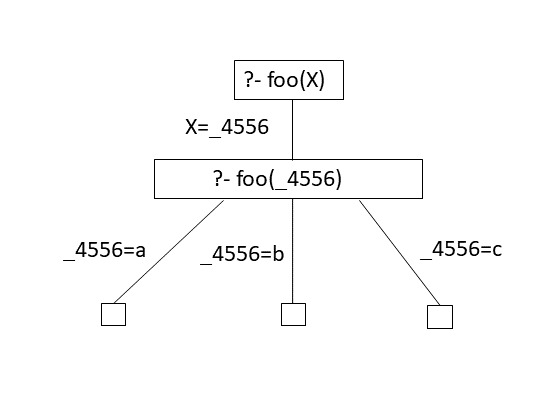
\includegraphics[width=0.4\textwidth]{images/foo4}

\begin{center}
\intens{arborele de căutare}
\end{center}
\end{figure}
\end{multicols}


\end{frame}


%-------------------------------------------------------------------

%------------------------------------------------------------------
\begin{frame}[fragile]{Cum găsește Prolog răspunsul}

\textbf{\color{True} Exemplu.} 
\begin{multicols}{2}
Să presupunem că avem programul: 
\begin{verbatim}
bar(b). 
bar(c). 
baz(c).
\end{verbatim}
și că punem întrebarea: \\
{\color{blue}\texttt{?- bar(X),baz(X).}}
\columnbreak
\begin{figure}[h]
    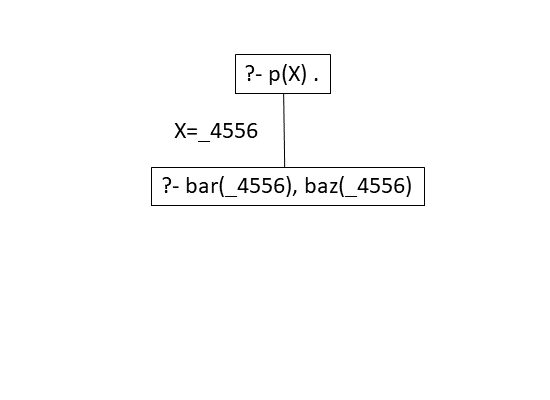
\includegraphics[width=0.4\textwidth]{images/bar1}
\end{figure}
\end{multicols}

\end{frame}

%------------------------------------------------------------------
\begin{frame}[fragile]{Cum găsește Prolog răspunsul}


\intens{Prolog se întoarce la ultima alegere dacă o subțintă eșuează.}

\textbf{\color{True} Exemplu.} 
\begin{multicols}{2}
Să presupunem că avem programul: 
\begin{verbatim}
bar(b). 
bar(c). 
baz(c).
\end{verbatim}
și că punem întrebarea: \\
{\color{blue}\texttt{?- bar(X),baz(X).}}
\columnbreak
\begin{figure}[h]
    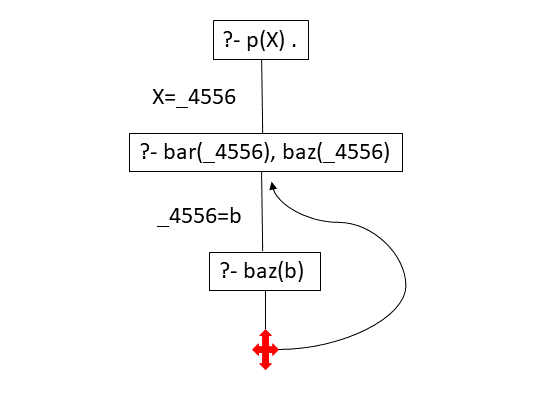
\includegraphics[width=0.4\textwidth]{images/bar2}
\end{figure}
\end{multicols}

\end{frame}


%------------------------------------------------------------------
\begin{frame}[fragile]{Cum găsește Prolog răspunsul}


\textbf{\color{True} Exemplu.} 
\begin{multicols}{2}
Să presupunem că avem programul: 
\begin{verbatim}
bar(b). 
bar(c). 
baz(c).
\end{verbatim}
și că punem întrebarea: \\
{\color{blue}\texttt{?- bar(X),baz(X).}}
\columnbreak
\begin{figure}[h]
    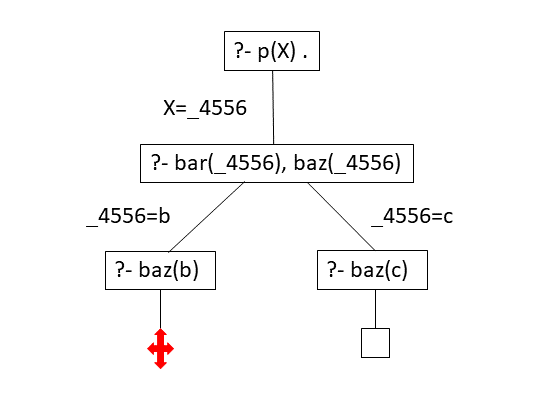
\includegraphics[width=0.4\textwidth]{images/bar3}
\end{figure}
\end{multicols}

\medskip

Soluția găsită este: \texttt{X=\_4556=c}.
\end{frame}

%--------------------------------------------------------------

\begin{frame}[fragile]{Cum găsește Prolog răspunsul}

\medskip
Ce se  întâmplă dacă schimbăm ordinea regulilor?

\textbf{\color{True} Exemplu.} 

Să presupunem că avem programul: 
\begin{verbatim}
bar(c). 
bar(b). 
baz(c).
\end{verbatim}
și că punem întrebarea: \\
{\color{blue}\texttt{?- bar(X),baz(X).}}\\
\pause
{\color{blue}\texttt{X = c ;}}\\
{\color{red}\texttt{false}}


\medskip

Vă explicați ce s-a întâmplat? Desenați arborele de căutare!

\end{frame}

%------------------------------------------------------------------
\begin{frame}[fragile]{Problema colorării hărților}

\intens{Să se coloreze o hartă dată cu o mulțime de culori dată astfel încât oricare două țări vecine să fie colorate diferit.}

\intens{Cum modelăm această problemă în Prolog?}
 
 \pause
\begin{multicols}{2}

Trebuie să definim:
\begin{itemize}
\item culorile
\item harta
\item constr\^{a}ngerile
\end{itemize}
\columnbreak
\begin{figure}[h]
    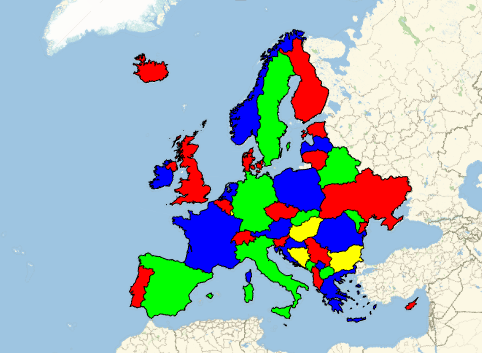
\includegraphics[width=0.4\textwidth]{images/europe1}
    
    \href{https://www.wolfram.com/mathematica/new-in-10/entity-based-geocomputation/find-the-shortest-route-through-the-worlds-capital.html}
    {\footnotesize{\intens{Sursa imaginii}}}
\end{figure}
\end{multicols}


\end{frame}

%\setbeamercolor*{block title}{fg=white, bg=MedianLightOrange}

%------------------------------------------------------------------
\begin{frame}[fragile]{Problema colorării hărților}

 \intens{Definim culorile, harta și constrângerile.}
 \onslide<2->{\intens{Cum punem întrebarea?}}


\vspace{-.3cm}
\begin{verbatim}
culoare(albastru).
culoare(rosu).
culoare(verde).
culoare(galben).

harta(RO,SE,MD,UA,BG,HU) :- vecin(RO,SE), vecin(RO,UA), 
                            vecin(RO,MD), vecin(RO,BG),                      	                          
                            vecin(RO,HU), vecin(UA,MD),
                            vecin(BG,SE), vecin(SE,HU).
                            
vecin(X,Y) :- culoare(X), culoare(Y), X \== Y.                      
\end{verbatim}
\onslide<3->{\color{blue}\texttt{?- harta(RO,SE,MD,UA,BG,HU).}}

\end{frame}



%------------------------------------------------------------------
\begin{frame}[fragile]{Problema colorării hărților}


\intens{Ce răspuns primim?}


{\color{blue}\texttt{?- harta(RO,SE,MD,UA,BG,HU).\\
RO = albastru,\\
SE = UA, UA = rosu,\\
MD = BG, BG = HU, HU = verde}} \rule{0.6ex}{1.3ex}


\end{frame}

%%---------------------------------------------------------------------
%\begin{frame}{Compararea termenilor: \texttt{=},\texttt{\textbackslash=},
%\texttt{==},\texttt{\textbackslash==}}
%\medskip
%
%\begin{center}
%\begin{tabular}{cl}
%\intens{\texttt{T = U}} & reușește dacă există  o potrivire 
%               (termenii se unifică)\\
%\intens{\texttt{T \textbackslash= U}} & reușește dacă nu există o potrivire\\
%\intens{\texttt{T == U}} &  reușește dacă termenii sunt identici \\
%\intens{\texttt{T \textbackslash== U}} &  reușește dacă termenii sunt diferiți 
%              \end{tabular}
%              \end{center}
% 
%\begin{example}
%\vspace*{-0.2cm}
%\begin{alltt}
%\begin{tabular}{ll}
%?- X = Y.  & ?- X == Y .   \\
%X = Y. & \textcolor{red}{false} \\[0.2cm]
%?- p(X,q(Z)) = p(Y,X). & ?- p(X,Y) == p(X,Y).   \\
%X = Y, Y = q(Z). & \textcolor{red}{true}  \\[0.2cm]
%?- 2 = 1 + 1 & ?- 2 == 1 + 1  \\
%\textcolor{red}{false} & \textcolor{red}{false}  
%\end{tabular}
%\end{alltt}
%\vspace*{-0.2cm}
%\end{example}
%
%\begin{itemize}
%\item \^{I}n exemplul de mai sus, \intens{\texttt{1+1}} este privită ca o expresie, nu este evaluată. Există și  predicate care forțează evaluarea (e.g., \intens{\texttt{=:=}}).
%\end{itemize}
%\end{frame}
%
%%---------------------------------------------------------------------
%\begin{frame}[fragile]{Negarea unui predicat: \textcolor{purple}{\texttt{\textbackslash + pred(X)}}}
%\vspace*{0.3cm}
%\begin{example}
%\begin{verbatim}
%animal(dog). animal(elephant). animal(sheep).
%
%?- animal(cat).
%false
%?- \+ animal(cat).
%true
%\end{verbatim}
%\end{example}
% 
%
%\begin{itemize}
%	\item Clauzele din Prolog dau doar condiții suficiente, dar nu și necesare pentru ca un predicat să fie adevărat.
%	\item Pentru a da un răspuns pozitiv la o țintă, Prolog trebuie să construiască o "demonstrație" pentru a arată că mulțimea de fapte și reguli din program implică acea țintă.
%	\item Astfel, un răspuns \alert{\texttt{false}} nu înseamnă neapărat că ținta nu este adevărată, ci doar că \alert{Prolog nu a reușit să găsească o demonstrație}.	
%%		\item Totuși, dacă  \intens{specificăm complet o problemă} (adică specificăm toate cazurile posibile), atunci noțiunile de nedemonstrabil și fals coincid. Atunci un \texttt{false} e chiar un fals.
%\end{itemize}
%\end{frame}
%
%%---------------------------------------------------------------------
%\begin{frame}[fragile]{Operatorul \textcolor{purple}{\textbackslash +}}
%
%\begin{itemize}
%	\item  Negarea unei ținte se poate defini astfel:
%	
%	\begin{verbatim}
%    neg(Goal) :- Goal, !, fail.
%    neg(Goal)
%	\end{verbatim}
%
%unde  \alert{\texttt{fail/0}} este un predicat care eșuează  întotdeauna.
% 
%\item \^{I}n PROLOG acest predicat este predefinit sub numele {\texttt {\textbackslash +}}. 
%\item Operatorul  \texttt{\textbackslash +} se foloseste pentru a nega un predicat.
%	\item \intens{\texttt{!}(cut)} este un predicat predefinit (de aritate 0) care restricționează mecanismul de backtracking:   execuția subțintei \texttt{!} se termină  cu succes, deci alegerile (instanțierile) făcute   înainte de a se ajunge la \texttt{{!}}  nu mai pot fi schimbate.
%	
%\item O țintă \texttt{\textbackslash + Goal} reușește dacă Prolog nu găsește o demonstrație pentru \texttt{Goal}. Negația din Prolog este definită ca incapacitatea de a găsi o demonstrație.
%
%	\item Semantica operatorului \texttt{{\textbackslash +}} se numește \textcolor{purple}{negation as failure}.
%
%\end{itemize}
%
%
%\end{frame}
%
%%---------------------------------------------------------------------
%\begin{frame}[fragile]{Negația ca eșec ("negation as failure")}
%
%\begin{example}
%Să presupunem că avem o listă de fapte cu perechi de oameni căsătoriți între ei:
%
%\begin{verbatim}
%married(peter, lucy).
%married(paul, mary).
%married(bob, juliet).
%married(harry, geraldine).
%\end{verbatim}
%\end{example}
%\end{frame}
%
%%---------------------------------------------------------------------
%\begin{frame}[fragile]{Negația ca eșec}
%
%\begin{example}[cont.]
%Putem să definim un predicat \texttt{\intens{single/1}} care reușește dacă argumentul său nu este nici primul nici al doilea argument în faptele pentru \texttt{married}.
%
%\begin{verbatim}
%single(Person) :-
%       \+ married(Person, _),
%       \+ married(_, Person).
%\end{verbatim}
%
%\begin{tabular}{lll}
%\texttt{?- single(mary).} &  \texttt{?- single(anne).}  &  \texttt{?- single(X).} \\
%\texttt{false}  & \texttt{true} & \texttt{false}
%\end{tabular}
%
%\bigskip
%Răspunsul la întrebarea \texttt{?- single(anne).} trebuie g\^andit astfel:
%\begin{center}
%{\em Presupunem că Anne este single, \\ deoarece \intens{nu am putut demonstra} că este maritată.}
%\end{center}
%\end{example}
%\end{frame}
%
%
%\begin{frame}[fragile]{Predicatul \texttt{->} /2 (\texttt{if-then-else})}
%
%\begin{itemize}
%	\item  \texttt{if-then}
%	
%	\begin{verbatim}
%     If -> Then :- If, !, Then.
%	\end{verbatim}
%	 
%	
%	\item  \texttt{if-then-else}
%	
%	\begin{verbatim}
%    If -> Then; _Else :- If, !, Then.
%    If -> Then; Else :- !, Else.
%	\end{verbatim}
%	
%Se încearcă demonstrarea predicatului \texttt{If}. Dacă întoarce true atunci se încearcă demonstrarea predicatului \texttt{Then}, iar dacă întoarce false se încearcă demonstrarea predicatului \texttt{Else}.	
%\end{itemize}
%
%\begin{verbatim}
%max(X,Y,Z) :- (X =< Y) -> Z = Y ;  Z = X  
%\end{verbatim}
%
%\begin{alltt}
%?- max(2,3,Z).
%Z = 3.
%\end{alltt}
%
%\medskip 
%
%Observăm că  \texttt{If -> Then} este  echivalent cu 
%\texttt{If -> Then ; fail}.
%\end{frame}
%

\begin{frame}{Liste în Prolog}
\begin{itemize}
\item O listă  în Prolog este un șir de elemente, separate prin virgulă,  între paranteze drepte:

\begin{center}
\intens{\texttt{[1,cold, parent(jon),[winter,is,coming],X]}}
\end{center}
\item O listă poate conține termeni de orice fel.
\item Ordinea termenilor din listă are importanță:
\begin{alltt}
?- [1,2] == [2,1] .\\
\alert{false}
\end{alltt}
\item Lista vidă se notează \intens{[$ \, $]}.
\item Simbolul \intens{$\mid$} desemnează coada listei:
\begin{alltt}
?- [1,2,3,4,5,6] = [X|T]. \\
X = 1, T = [2, 3, 4, 5, 6].\\
\medskip
?- [1,2,3|[4,5,6]] == [1,2,3,4,5,6].\\
true.
\end{alltt}
\end{itemize}
\end{frame}

%\begin{frame}{Listă \texttt{[t1,\ldots,tn]==[t1 |[t2,\ldots,tn]}}
%\begin{itemize}
%\item Simbolul \intens{$\mid$} desemnează coada listei:
%\begin{alltt}
%?- [1,2,3,4,5,6] = [X|T]. \\
%X = 1, \\
%T = [2, 3, 4, 5, 6].
%\end{alltt}
%
%\item Variabila anonimă \intens{\texttt{\_}} este unificată cu orice termen Prolog:
%\begin{alltt}
%?- [1,2,3,4,5,6] = [X|\_]. \\
%X = 1.
%\end{alltt}
%
%\item Deoarece Prologul face unificare poate identifica șabloane mai complicate: 
%\begin{alltt}
%?- [5,1,1,3,2]=[\_|[X|[X|\_]]].\\
%X = 1.
%
%?- [5,1,4,3,2]=[\_|[X|[X|\_]]].\\
%false.
%\end{alltt}
%\end{itemize}
%\end{frame}

\begin{frame}{Liste în Prolog}


\textbf{\color{True} Exerciții.}

\begin{enumerate}
\item  Definiți un predicat care verifică că un termen este lista.

 \pause
\begin{alltt}
is\_list([]).\\
is\_list([\_ | T]) :- is\_list(T).
\end{alltt}
 
\pause \vspace{.2cm}
\item Definiți predicate care verifică dacă un termen este primul element, ultimul element sau coada unei liste.

\pause
\begin{alltt}
head([X|\_],X). \\

last([X],X). \\
last([\_|T],Y):- last(T,Y).\\
 
tail([],[]).\\
tail([\_|T],T).
\end{alltt}
\end{enumerate}
\end{frame}

%\begin{frame}{Liste}
%\vspace*{0.3cm}
%
%\begin{block}{Exercițiu}
%\begin{itemize}
%
%\item Definiți un predicat care verifică dacă un termen aparține unei liste.
% 
%\begin{alltt}
%member(H, [H|\_]).\\
%member(H, [\_|T]) :- member(H,T).
%\end{alltt}
%
%
%\medskip 
%
%\item Definiți un predicat \texttt{append/3} care verifică dacă o listă se obține prin concatenarea altor două liste.
% 
%\begin{alltt}
%append([],L,L).\\
%append([X|T],L, [X|R]) :- append(T,L,R).\\
%\end{alltt}
%
%\end{itemize}
%\end{block}
%
% 
%Există predicatele predefinite \intens{\texttt{member/2}} și 
%\intens{\texttt{append/3}}. 
%\end{frame}

%\begin{frame}{Liste \texttt{append/3}}
%
%\vspace*{0.3cm}
%
%\begin{itemize}
%\item Funcția \texttt{append/3}:
%\begin{alltt}
%?- listing(append/3).\\
%append([],L,L).\\
%append([X|T],L, [X|R]) :- append(T,L,R).\\
%
%?- append(X,Y,[a,b,c]).\\
%X = [],\\
%Y = [a, b, c] ;\\
%X = [a],\\
%Y = [b, c] ;\\
%X = [a, b],\\
%Y = [c] ;\\
%X = [a, b, c],\\
%Y = [] ;\\
%\alert{false}
%\end{alltt}
%\item Funcția astfel definită poate fi folosită 
%at\^ at pentru verificare, c\^ at și pentru generare. 
%\end{itemize}
%
%
%\end{frame}

%\begin{frame}{Liste}
%\vspace*{0.3cm}
%
%\begin{block}{Exercițiu}
%\begin{itemize}
%\item Definiți un predicat \texttt{elim/3} care verifică dacă o  listă se obține din alta prin eliminarea unui element.
%\medskip 
%\begin{alltt}
%elim(X, [X|T], T).\\
%elim(X, [H|T], [H|L]) :- elim(X,T,L).
%\end{alltt}
%
%
%\medskip 
%
%\item Definiți un predicat care \texttt{perm/2} care verifică dacă două liste sunt permutări.
%\medskip 
%\begin{alltt}
%perm([],[]). \\
%perm([X|T],L) :- elim(X,L,R), perm(R,T).
%\end{alltt}
%
%\end{itemize}
%\end{block}
% 
%Predicatele predefinite \intens{\texttt{select/3}} și 
%\intens{\texttt{permutation/2}} au aceeași funcționalitate. 
%\end{frame}

%\begin{frame}{Generează și testează}
%\vspace*{0.3cm}
%
%\begin{center}
%\intens{\texttt{solution(X) :- generate(X), check(X).}}
%\end{center}
%
%\begin{block}{Exercițiu}
%Determinați toate cuvintele dintr-o bază de 
%cunoștințe dată, care sunt anagrame ale unui cuv\^ ant dat.
%
%\medskip
%
%KB: \texttt{word(relay). word(early). word(layer).}
%\medskip
%
%Predicat util:\\
%\begin{alltt}
%?- name(relay,L). \% {\em conversie  între atomi și liste}\\
%L = [114, 101, 108, 97, 121]
%\end{alltt}
%\end{block}
% 
%Două abordări posibile:
%\begin{itemize}
%\item  se generează o posibilă soluție apoi se testează dacă este  în KB.
%\item se parcurge KB și pentru fiecare termen se testează dacă e soluție. 
%\end{itemize}
%\end{frame}
%
%\begin{frame}{Generează și testează}
%\vspace*{0.2cm}
%
%\begin{center}
%\intens{\texttt{solution(X) :- generate(X), check(X).}}
%\end{center}
%
%\vspace*{-0.2cm}
%\begin{block}{Exercițiu}
%Determinați toate cuvintele dintr-o bază de 
%cunoștințe dată, care sunt anagrame ale unui
% cuv\^ ant dat.
%\medskip
%
%KB: \texttt{word(relay). word(early). word(layer).}
%\medskip
%
% 
%\begin{alltt}
%anagram1(A,B) :- name(A,L), permutation(L,W), \\
%\hspace*{3.1cm}name(B,W), word(B).\\  
%anagram2(A,B) :-  name(A,L), word(B), \\
%\hspace*{3.1cm}name(B,W),  permutation(L,W).\\
%\end{alltt}
% 
%
%\vspace*{-0.2cm}
%\begin{columns}
%\begin{column}{0.45\textwidth}
%\begin{alltt}
%?- anagram1(layre,X).\\
%X = layer ;\\
%X = relay ;\\
%X = early ;\\
%\alert{false.}
%\end{alltt}
%\end{column}
%\begin{column}{0.45\textwidth}
%\begin{alltt}
%?- anagram2(layre,X).\\
%X = relay ;\\
%X = early ;\\
%X = layer ;\\
%\alert{false.}
%\end{alltt}
%\end{column}
%\end{columns}
%\end{block}
%\end{frame}
%
%
%\begin{frame}{Recursie}
%\vspace*{0.3cm}
%
%\begin{block}{Exercițiu}
%\begin{itemize}
%
%\item Definiți un predicat \texttt{rev/2} care verifică dacă o listă este inversa altei liste. 
%\medskip 
%\begin{alltt}
%rev([],[]).\\
%rev([X|T],L) :- rev(T,R),append(R,[X],L).
%\end{alltt}
%\end{itemize}
%\end{block}
%
%Soluția de mai sus este corectă, dar foarte costisitoare computațional, datorită stilului de programare declarativ. 
%\medskip
%
%
%\intens{Cum putem defini o variantă mai rapidă?}
%
%\medskip
%
%O metodă care prin care recursia devine mai rapidă este folosirea \intens{acumulatorilor},  în care se păstrează rezultatele parțiale.
% 
%\end{frame}
%
%\begin{frame}{Recursie cu acumulatori}
%\begin{itemize}
%\item Varianta inițială:
%\begin{alltt}
%rev([],[]).\\
%rev([X|T],L) :- rev(T,R),append(R,[X],L). 
%\end{alltt}
%\item Varianta cu acumulator
%\begin{alltt}
%rev(L,R) :- revac(L,\intens{[]},R).\\
%\% {\em la momentul inițial nu am acumulat nimic.  }    
%\medskip 
%
%revac([], \intens{R}, R).\\
%\% {\em cand lista inițială a fost consumată,}\\
%\% {\em am acumulat rezultatul final.}
%\medskip 
%
%revac([X|T], \intens{Acc}, R) :- revac(T,\intens{[X|Acc]},R).\\
%\% \texttt{Acc} {\em conține inversa listei care a fost deja parcursă.} 
%\end{alltt}
%\item Complexitatea a fost redusă de la $O(n^2)$ la $O(n)$, unde $n$ este lungimea listei.
%\end{itemize}
%\end{frame}
%
%%\begin{frame}{Recursie}
%%
%%\begin{itemize}
%%\item Multe implementări ale limbajului Prolog aplică "{\em last call optimization}" atunci c\^ and un apel recursiv este ultimul predicat din corpul unei clauze ({\em tail recursion}).
%%
%%\medskip
%%\item Atunci c\^ and este posibil, se recomandă utilizare recursiei la coadă ({\em tail recursion}).
%%
%%\medskip
%%\item Vom defini un predicat care generează liste lungi  în două moduri și vom analiza performanța folosind predicatul \intens{time/1}.
%%\end{itemize}
%%
%% 
%%\begin{alltt}
%%biglist(0,[]).\\
%%biglist(N,[N|T]) :- N >= 1, M is N-1,biglist(M,T),M=M.\\
%%
%%biglist\_tr(0,[]).\\
%%biglist\_tr(N,[N|T]) :- N >= 1, M is N-1,biglist\_tr(M,T).
%%\end{alltt}
%%
%%
%%\end{frame}
%%
%%\begin{frame}{Recursie la coadă}
%%
%%\vspace*{0.5cm}
%%
%%\begin{itemize}
%%\item Predicat \textcolor{magenta}{fără} recursie la coadă:
%%\begin{alltt}
%%biglist(0,[]).\\
%%biglist(N,[N|T]) :- N >= 1, M is N-1,biglist(M,T),\textcolor{magenta}{M=M}.
%%\end{alltt}
%%
%%Apelul recursiv  întoarce valoarea găsită  în predicatul apelant, acestă valoare urm\^{a}nd a fi prelucrată.  
%%
%%\begin{alltt}
%%?- time(biglist(50000,X)).\\
%%\intens{ 100,000 inferences, 0.016 CPU in 0.038 seconds \\
%%(41\% CPU, 6400000 Lips)}\\
%%X = [50000, 49999, 49998|...] .
%%\end{alltt} 
%%
%%\item Predicatul \intens{cu} recursie la coadă:
%%\begin{alltt}
%%biglist\_tr(0,[]).\\
%%biglist\_tr(N,[N|T]) :- N >= 1, M is N-1,biglist\_tr(M,T).\\
%% 
%%
%%?- time(biglist\_tr(50000,X)).\\
%%\intens{100,000 inferences, 0.000 CPU in 0.007 seconds \\(0\% CPU, Infinite Lips)}\\
%%X = [50000, 49999, 49998|...]
%%\end{alltt} 
%%
%%\end{itemize}
%%\end{frame}
%%
%
%
%%\begin{frame}{Liste}
%%\begin{alltt}
%%append([],L,L).\\
%%append([X|T],L, [X|R]) :- append(T,L,R).\\
%%\end{alltt}
%%
%%
%%\begin{block}{Exercițiu}
%% Definiți \intens{\texttt{prefix/2}} și \intens{\texttt{suffix/2}} folosind \texttt{append}.
%% 
%%
%%\begin{alltt}
%%prefix(P,L) :- append(P,\_, L).\\
%%suffix(S,L)  :- append(\_,S,L).\\
%%\end{alltt} 
%%\end{block}
%% 
%%
%%Observăm că funcția \texttt{append} parcurge prima listă.
%%\medskip
%%
%%\intens{Am putea rescrie această funcție astfel  înc\^ at legătura să se facă direct, așa cum putem face  în programarea imperativă?}
%%
%%\medskip 
%%
%%Problema poate fi rezolvată scriind \intens{listele ca diferențe}, o tehnică utilă  în limbajul Prolog.
%%\end{frame}
%%
%%\begin{frame}{Liste ca diferențe}
%%\begin{itemize}
%%\item Ideea:  lista \texttt{[t1,\ldots,tn]} va fi reprezentată printr-o pereche 
%%\begin{center}
%%\intens{\texttt{([t1,\ldots,tn|T], T)}}
%%\end{center}
%%
%%Această pereche poate fi notată \intens{\texttt{[t1,\ldots,tn|T]- T}}, dar notația nu este importantă. 
%%
%% 
%%
%%\item Vrem să definim \texttt{append/3} pentru liste ca diferențe:
%%
%%\medskip
%%
%%\texttt{\intens{dlappend((X1,T1),(X2,T2),(R,T)) :-} \alert{?}.} 
%%
%%\end{itemize}
%%
%%
%% 
%%\begin{alltt}
%%?- dlappend(([1,2,3|P],P),([4,5|T],T),RD).\\
%%P = [4, 5|T],\\
%%RD =  ([1, 2, 3, 4, 5|T], T).\\
%%\end{alltt}
%%
%%\end{frame}
%%
%%\begin{frame}{Liste ca diferențe \texttt{([t1,\ldots,tn|T], T)}}
%% \medskip
%% 
%% \texttt{dlappend((X1,T1),(X2,T2),(R,T)) :- \alert{?}.} \\
%%
%% \medskip
%%
%%\begin{itemize}
%%\item Dacă \texttt{[t1,\ldots, tn]} este diferența \texttt{(X1,T1)}, iar \texttt{[q1,\ldots, qk]} este diferența \texttt{(X2,T2)} observăm că diferența \texttt{(R,T)} trebuie să fie  \texttt{[t1,\ldots,tn,q1\ldots, qk]}.  
%%\item  Obținem  \texttt{R=[t1,\ldots,tn,q1\ldots, qk|T]}, deci 
%%
%%\texttt{(X1,T1) = (R, P)}  și  \texttt{(X2,T2) = (P,T)}
%%
%%unde \texttt{P =[q1,\ldots,qk|T])}. 
%%
%%\item Definiția este:
%%\begin{center}
%%\texttt{\intens{dlappend((R,P),(P,T),(R,T)).}}
%%\end{center}
%%\end{itemize}
%% 
%%\begin{alltt}
%%?- dlappend(([1,2,3|P],P),([4,5|T],T),RD).\\
%%P = [4, 5|T],\\
%%RD =  ([1, 2, 3, 4, 5|T], T).\\
%%\end{alltt}
%% 
%%
%%\begin{itemize}
%%\item \texttt{dlappend} este foarte rapid, dar nu poate fi folosit pentru generare, ci numai pentru verificare. 
%%\end{itemize}
%%\end{frame}
%
%
%%-------------------------------------------------------------
%\section{Tipuri de date compuse} \sectionframe
%%-------------------------------------------------------------
%\begin{frame}{Termeni compuși \texttt{f(t1,$\ldots$, tn)}}
%\begin{itemize}
%	\item \intens{Termenii} sunt unitățile de bază prin care Prolog reprezintă datele.
%	\smallskip
%	\item Sunt de 3 tipuri:
%	\begin{itemize}
%		\smallskip
%		\item \intens{Constante}:
%		 \texttt{23, sansa, 'Jon Snow'}
%		\smallskip
%		\item \intens{Variabile}: \texttt{X, Stark, \_house}
%		\smallskip
%		\item \intens{Termeni compuși:}
%\begin{itemize}
%\item predicate
%\item termeni prin care reprezentăm datele 		\end{itemize}
%\end{itemize}
%\end{itemize}
%\begin{example}
%\begin{itemize}
%\item \texttt{born(john, date(20,3,1977))}
%\begin{itemize}
%\item \texttt{born/2} și \texttt{date/3} sunt {\em functori}
%\item \texttt{born/2} este un predicat
%\item \texttt{date/3} definește  date compuse 
%\end{itemize}
%
%\end{itemize}
%\end{example}
%\end{frame}
%
%
%\begin{frame}{Tipuri de date definite recursiv}
%\begin{itemize}
%\item Am văzut că listele sunt definite recursiv astfel:
%\medskip
%
%\begin{itemize}
%\item \texttt{[]} este listă
%\item \texttt{[X|L]} este listă, unde \texttt{X} este element și \texttt{L} este listă
%\end{itemize}
%
%\bigskip 
%
%\item Cum definim arborii binari  în Prolog?   Soluție posibilă: 
%\medskip
%
%\begin{itemize}
%\item \texttt{void} este arbore  
%\item \texttt{tree(X,A1,A2)} este arbore, unde \texttt{X} este un element, iar \texttt{A1} și \texttt{A2} sunt arbori
%\end{itemize} 
%\end{itemize}
% 
%
%\begin{center}
%\intens{\texttt{tree(X,A1,A2)}} este un termen compus, dar nu este un predicat!
%\end{center}
%\end{frame}
%
%\begin{frame}{Arbori binari  în Prolog}
%
%\begin{itemize}
%\item Cum arată un arbore?  
%
%\begin{center}
%\mbox{\intens{tree(a, tree(b, tree(d, void, void), void), tree(c, void, tree(e, void, void)))}}
%\end{center}
%
%\bigskip 
%
%\item Cum dăm un "nume" arborelui de mai sus?    \quad Definim un predicat:
%
%\begin{alltt}
%
%
%\intens{def(arb, tree(a, tree(b,\\
%      \hspace*{4.5cm}                   tree(d,void,void),\\
%       \hspace*{4.5cm}                  void),\\
%       \hspace*{3cm}          tree(c, void,\\
%        \hspace*{4.5cm}                 tree(e,void,void)))).}
%\end{alltt}
%\end{itemize}
% 
%\medskip
%
% Deoarece  în  Prolog nu avem  declarații explicite de date, pentru a defini arborii vom scrie un predicat care este adevărat atunci c\^ and argumentul 
%său este un arbore.
%\end{frame}
%
%
%\begin{frame}{Arbori binari  în Prolog}
%
%\vspace{.5cm}
%Scrieți un predicat care verifică că un termen este arbore binar. 
%
%
% 
%
%\begin{alltt}
%binary\_tree(void).\\
%binary\_tree(tree(Element,Left,Right)) :- \\
%\hspace*{5cm}binary\_tree(Left), \\
%\hspace*{5cm}binary\_tree(Right).
%\end{alltt}
%
% 
%Eventual putem defini și un predicat pentru elemente:
%
%\begin{alltt}
%binary\_tree(void).\\
%binary\_tree(tree(Element,Left,Right)) :-  \\
%\hspace*{5cm}binary\_tree(Left), \\
%\hspace*{5cm}binary\_tree(Right), \\ 
%\hspace*{5cm}element\_binary\_tree(Element). \\
%
%element\_binary\_tree(X):- integer(X). /* de exemplu */\\
%
% 
%test:- def(arb,T), binary\_tree(T). 
%
%\end{alltt}
%\end{frame}
%
%\begin{frame}{Arbori binari  în Prolog}
%\begin{block}{Exercițiu}
%
%Scrieți un predicat  care verifică dacă un element aparține unui arbore.
%\medskip  
%
%\begin{alltt}
%tree\_member(X,tree(X,Left,Right)). \\
%
%tree\_member(X,tree(Y,Left,Right)) :- tree\_member(X,Left). \\
%	
%tree\_member(X,tree(Y,Left,Right)) :- tree\_member(X,Right).
%\end{alltt}
%\end{block}
%\end{frame}
%
%
%%\begin{frame}{Arbori binari  în Prolog}
%%\begin{block}{Exercițiu}
%%
%%Scrieți un predicat  care verifică că  doi arbori binari sunt izomorfi (fiecare nod are acceași copii, dar ordinea nu contează).
%%
%%\bigskip 
%%\begin{alltt}
%%isotree(void,void).\\
%%\medskip
%%
%%isotree(tree(X,Left1,Right1),tree(X,Left2,Right2)) :- 
%%
%%	\hfill	isotree(Left1,Left2), isotree(Right1,Right2).
%%
%%\medskip
%%
%%	isotree(tree(X,Left1,Right1),tree(X,Left2,Right2)) :- 
%%
%%\hfill isotree(Left1,Right2), isotree(Right1,Left2).
%%\end{alltt}
%%\end{block}
%%\end{frame}
%
%
%\begin{frame}{Arbori binari  în Prolog}
%
%\vspace{.4cm}
%\begin{block}{Exercițiu}
%
%Scrieți un predicat  care determină parcurgerea  în preordine a unui arbore binar. 
%
% 
%\begin{alltt}
%
%preorder(tree(X,L,R),Xs) :-	 preorder(L,Ls),
%
%\hspace*{5cm} preorder(R,Rs), 
%
%\hspace*{5cm}		append([X|Ls],Rs,Xs).
%
%preorder(void,[]).
%
%
%
%test(Tree,Pre):- def(arb, Tree), preorder(Tree,Pre).
%\medskip
%  
%
%?- test(T,P).\\
%T = tree(a, tree(b, tree(d, void, void), void), tree(c, void, tree(e, void, void))),\\
%P = [a, b, d, c, e]
%\end{alltt}
%\end{block}
%
%
%\end{frame}

%%------------------------------------------------
%\begin{frame}
%  \vfill
%  \centering
%
%TODO
%
%\textbf{\large \alert{Quiz time!}}
%
%
\includegraphics[scale=.35]{../Quiz/C06-Q1.png}
%
% \url{https://www.questionpro.com/t/AT4NiZrPCD}
%  \vfill
%\end{frame}



%---------------------------------------------
\begin{frame}
  \vfill
  \centering

\textbf{Pe data viitoare!}

  \vfill
\end{frame}
\end{document}







